% !TEX TS-program = pdflatex
% !TEX encoding = UTF-8 Unicode

\documentclass{beamer}
\usepackage[czech]{babel}
\usepackage[utf8]{inputenc}
\usepackage{times}
\usepackage[T1]{fontenc}
\usepackage{verbatim}
\usepackage{listings}
\usepackage{xcolor}

\mode<presentation>
{
	\usetheme{antibes}
	\usecolortheme{orchid}
}

\setbeamertemplate{navigation symbols}{}

\definecolor{cmtgreen}{RGB}{0,192,0}

\begin{document}

\title{C++; delete Java;}
\subtitle{Část 9: šablony}
\author{Kennny}
\date{srpen 2017}

\frame{\titlepage}

\lstset{language=C++,
        basicstyle=\ttfamily,
        keywordstyle=\color{blue}\ttfamily,
        stringstyle=\color{red}\ttfamily,
        commentstyle=\color{cmtgreen}\ttfamily,
        morecomment=[l][\color{magenta}]{\#}
}

\newenvironment{xframe}[1][]
  {\begin{frame}[fragile,environment=xframe,#1]}
  {\end{frame}}

\begin{comment}
\begin{xframe}{tttt}
	\begin{itemize}
		\item
	\end{itemize}
\end{xframe}
\end{comment}



\section{Šablony}
\subsection{Úvod}



\begin{xframe}{Šablony}
	\begin{itemize}
		\item princip, který dovoluje vytvářet více variant implementace z jedné předlohy
		\item implementační "mezikrok"~generické implementace
		\item nemělo by nahrazovat dědičnost, polymorfismus a další principy OOP
	\end{itemize}
	
	\begin{figure}
		\centering
		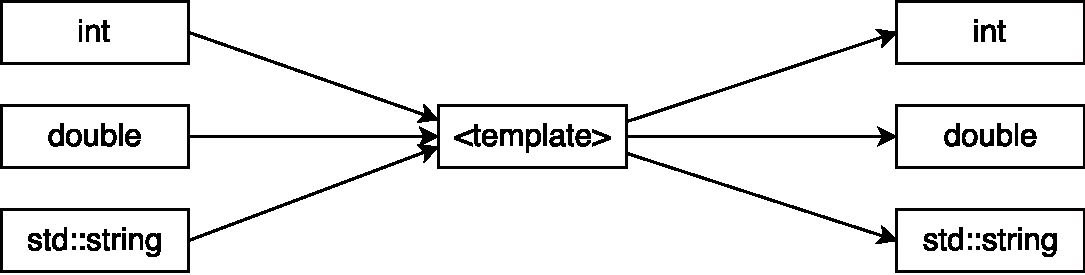
\includegraphics[width=0.6\textwidth]{templschema.pdf}
	\end{figure}
\end{xframe}


\begin{xframe}{Šablony}
	\begin{itemize}
		\item šablonová může být funkce (metoda) a třída
		\item klíčové slovo \texttt{template} a \texttt{typename}
		\item přibyde symbol, kterým nahrazujeme typ
\begin{lstlisting}[basicstyle=\fontsize{8}{9}\selectfont\ttfamily]
template<typename T>
void DoSomething(T& input)
{
    // ...
}
\end{lstlisting}
		\item při volání buď kompilátor rozhodne, co za typ dosadí, nebo můžeme explicitně uvést
\begin{lstlisting}[basicstyle=\fontsize{8}{9}\selectfont\ttfamily]
DoSomething(5); // pravdepodobne T = int
DoSomething<double>(5); // T = double
\end{lstlisting}
	\end{itemize}
\end{xframe}

\begin{xframe}{Šablony}
	\begin{itemize}
		\item při překladu se šablona specializuje tak, aby vyhověla všem voláním
\begin{lstlisting}[basicstyle=\fontsize{8}{9}\selectfont\ttfamily]
void DoSomething(int& input)
{
    // ...
}

void DoSomething(double& input)
{
    // ...
}
\end{lstlisting}
	\end{itemize}
\end{xframe}

\begin{xframe}{Explicitní specializace}
	\begin{itemize}
		\item pokud nechceme specializaci nechat na kompilátoru, můžeme specializovat explicitně
\begin{lstlisting}[basicstyle=\fontsize{8}{9}\selectfont\ttfamily]
template<>
void DoSomething<double>(double& input)
{
    // ...
}
\end{lstlisting}
		\item kompilátor pak nebude vytvářet novou specializaci, ale použije naši
	\end{itemize}
\end{xframe}

\begin{xframe}{Jednoduchý příklad}
	\begin{itemize}
		\item příkladem použití může být například potřeba vytisknout něco v řádce - víme že budeme pracovat se spoustou typů, nemůžeme tedy implementovat X různých variant
		\item zároveň ale víme, že std::cout se už umí chovat podle vstupního typu
\begin{lstlisting}[basicstyle=\fontsize{8}{9}\selectfont\ttfamily]
template<typename T>
void printLine(T& input)
{
    std::cout << input << std::endl;
}
\end{lstlisting}
	\end{itemize}
\end{xframe}


\begin{xframe}{Příklad}
	\begin{itemize}
		\item Prostor pro příklad 09\_a\_templates
	\end{itemize}
\end{xframe}




\begin{xframe}{Konec 9. části}
\texttt{exit(0);}
\end{xframe}




\end{document}




